\documentclass[a4paper,11pt,pdftex,halfparskip,cleardoubleempty]{scrbook}

\raggedbottom

% \usepackage{fancyhdr}

\usepackage[utf8]{inputenc}
\usepackage{wrapfig}
\usepackage[pdftex]{graphicx}
\usepackage{eso-pic}
\usepackage{array}
\usepackage{tabularx}
\usepackage{float}
\usepackage{listings}

\setlength{\tabcolsep}{20pt}
\renewcommand{\arraystretch}{4}

\graphicspath{{img/}}
\newcommand*{\xchapter}{\stepcounter{chapter}\setcounter{section}{0}\addchap}
\renewcommand*{\thesection}{\arabic{section}}

% define medatata
\def\MTitle{High-Level Modeling and Low-Level Adaption of Serverless Function Choreographies}
\def\MAuthor{Benjamin Walch}
\def\MKeywords{Serverless \sep Function Choreography Language}
\def\MOrg{Universit{\"a}t Innsbruck}
\def\MDate{\today}
\def\MInstitution{Department of Computer Science}
\def\MSupervisor{Dr. Shashko Ristov}
\def\MGroup{Distributed and Parallel Systems}

%
% \pagestyle{fancy}
% \fancyhf{}
% \fancyhead[L]{\leftmark}
% \fancyhead[R]{\thepage}
% \fancyfoot[R]{B. Walch}
% \fancyfoot[L]{Fastlane}

\begin{document}

\frontmatter
\pagestyle{empty}

\begin{titlepage}
\rule{0mm}{1mm}

\begin{multicols}{2}[\columnsep2em] 
	
\includegraphics[width=6cm]{uibk-logo}
	\columnbreak
	\begin{flushright}
		\Large{\textsf{\MOrg}}
	\end{flushright}
\end{multicols}

\begin{flushright}
	{\large \MInstitution\\}
	{\large \MGroup}
\end{flushright}

\vspace*{1.5cm}

\begin{center}
	{\LARGE\bf \MTitle}
	\vskip 2.25cm
	\Large \textbf{Bachelor Thesis}
	\vskip 2.25cm
	{\Large \MAuthor}
	\vskip 1.5cm
	{\large Supervisor: \MSupervisor}   
	\vfill
	{\large Innsbruck, \MDate}
\end{center}
%\AddToShipoutPicture{
%	\put(-55,55){
%		\parbox[b]{\paperwidth}{
%			\hfill 
\includegraphics[scale=0.35]{uibk-watermark}
%		}
%	}
%}
\end{titlepage} 

\ClearShipoutPicture

\cleardoublepage

\section*{Eidesstaatliche Erklärung}

Ich erkläre hiermit an Eides statt durch meine eigenhändige Unterschrift, dass ich die vorliegende Arbeit selbständig verfasst und keine anderen als die angegebenen Quellen und Hilfsmittel verwendet habe. Alle Stellen, die wörtlich oder inhaltlich den angegebenen Quellen entnommen wurden, sind als solche kenntlich gemacht.

Ich erkläre mich mit der Archivierung der vorliegenden Bachelorarbeit einverstanden.

\vspace{1.8cm}

\parbox{6cm}{
	\hrule
	\strut \centering\footnotesize Datum
} \hfill
\parbox{6cm}{
	\hrule
	\strut \centering\footnotesize Unterschrift
}

\cleardoublepage

\pagenumbering{arabic}
\pagestyle{plain}

\section*{Abstract}
In the FaaS world, there exist many providers who offer serverless execution of code (functions) in the cloud. Each of them has its own specifications and definitions on how functions are deployed and executed, and how workflows are created and executed.
\par
The Distributed and Parallel Systems group developed the "Abstract Function Choreography Language" (AFCL). It is a specification for describing serverless workflows. Also, a Java API, to describe serverless application workflows programmatically was developed.
The product which results in using that API is the workflow being described in AFCL in a text file.
Until now, the workflow described in the text file has to be created manually (by editing the file directly), or a programmer has to write Java code which utilizes the API to generate the file.
\par
The aim of this bachelor project is to develop a visual workflow editor, which makes modeling of workflows possible at a high level of abstraction. The tool should not only be able to load, display and save workflows, but also to optimize workflows for multiple \emph{FaaS} provider(s) in case of quotas and limits, and also in case of performance.

\cleardoublepage

\tableofcontents

\newpage

\section{Introduction}
"Run code, not Server" is the most recent term in the cloud computing environment.
With the rise of the serverless technology during the last years, \emph{FaaS} became more and more popular.
With the serverless technology, a high level of flexibility in execution of code became possible. Global Players like Amazon, Google, IBM and Microsoft jumped on the train and provide their infrastructure to Developers, able to deploy functions and execute them in the cloud. Each system has its own definitions on how to define, deploy and run a function. Many providers also offer a tool to model a workflow and execute it (Amazon Step Functions, IBM Cloud Functions, Microsoft Azure Functions, Google Cloud Functions, ...)

The distributed and parallel systems group developed a specification 

\label{sec:introduction}

\section{Background}

\subsection{FaaS}
\subsection{AFCL}

\section{Overview}

\section{Implementation}
The Implementation of a Graphical User Interface as well as the optimization for Workflows were the main goals of this bachelor thesis. 

\subsection{Requirements}

\begin{itemize}
	\item design for the overall application [coreUI]
	\item clean and intuitive UI [bootstrap]
	\item ability to add components/menu points easily [modularity]
	\item good user experience [SPA]
	\item frameworks: open source, large community (future-safe)
	\item cross-browser [?]
	\item performance [?]
\end{itemize}

\subsection{Frontend}
One of the main parts of the application is the frontend. Since a web based frontend which, runs in the user's web browser, is a hard requirement, the core technologies are limited to HTML, CSS and JavaScript.
\par
A prototyping phase was the kickoff for the development: Different frameworks and libraries have been researched, tested and selected. For the selection, the following criteria have been taken into account:
\begin{itemize}
	\item open-source
	\item good documentation
	\item large and active community (future-proof)
	\item stars on github / downloads on npmtrends
	\item performance
	\item pre-knowledge of the developer / learning curve
\end{itemize}
This criteria ensure the usage of well-documented and open-source software and makes it easier for others (dps) to extend the application later.
The result of this development phase was a working prototype as proof-of-concept.
In the following sections, the setup and each chosen technology and frameworks are described in detail.

% add definitions here (EcmaScript JavaScript SASS ...)

% \subsubsection{Development Workflow}
\subsubsection{Setup}

The setup of the frontend application is a selection of tools and technologies for modern and complex web development.
Under the hood, JavaScript and several JavaScript Frameworks are in action to control the application consisting of several UI components. To give the application its look and feel, CSS and some CSS Frameworks are in use.
The base forms the node package manager (npm) which is used to manage and resolve the dependencies. Additionally, npm's CLI is used as tool to execute development and build tasks. \\
Webpack does much of heavy-lifting, by bundling all sources with the assets into single files, and execute additional build steps by utilizing so-called 'loaders'.
Babel is used as such a webpack loader, for compiling the ECMAScript and React JSX source code to browser-compatible JavaScript.
The same applies for the CSS extension SASS, which is also integrated as a webpack loader, and is used to make the process of styling the user interface more efficient.

\begin{figure}[htbp]
  \centering
  \includegraphics[trim={0.8cm 8.2cm 3.0cm 1cm},scale=0.6]{frontend-setup}
  \caption{frontend development workflow}
\end{figure}
%%% TECHNOLOGIES / TOOLS %%%

\subsubsection{npm}

The node package manager\footnote{https://www.npmjs.org} is the world's largest software registry, where open-source software packages of developers and companies are shared all over the world. Over the last years, npm became a de-facto standard for package management in JavaScript development.

\subsubsection{webpack}

webpack is a module bundler, its main purpose is to bundle JavaScript code for the usage in a browser.\footnote{https://webpack.js.org} In particular, multiple modules (often hundreds of) with dependencies [to each other] are processed and bundled into a few files. To be able to process other types of files than JavaScript or JSON, webpack offers the opportunity to configure a \textbf{loader}. In this application, the following loaders are configured:
\begin{itemize}
\item babel-loader, to transform ECMAScript and React JSX to browser-compatible JavaScript
\item sass-loader, to transform SASS to CSS
\item css-loader, to transform CSS to CommonJS
\item file-loader, to handle static resources like images and fonts
\end{itemize}

\subsubsection{ECMAScript}

The scripting language specification ECMAScript (ES) was created to standardize JavaScript. With the release of ES6 (also known as ECMAScript 2015), features like class declarations, module imports and arrow function expressions became possible. After ES6, every year a new edition of the ECMAScript standard was finalized and released, offering new features. Worth mentioning here is the rest/spread operator released with ES9, which occurs a lot in the source code of this thesis.\\
% spread operator is a lot in use in source code
Since current browsers only have partial support of ECMAScript, a compile 'transcompiler' (or transpiler) is needed to transform the ECMAScript source code to JavaScript common browsers are capable of interpreting.
This process of compiling is done with Babel\footnote{https://babeljs.io}, which is configured to not only compile ECMAScript, but also JSX to JavaScript.

\subsubsection{SASS}

CSS, in its pure form, reaches its limits when one thinks about using variables, functions or nested rules. SASS\footnote{https://sass-lang.com} is a stylesheet language, which is compiled to CSS and offers the mentioned and even more features.
A lot of CSS Frameworks also offer its source code in SASS with a large variable set which makes it easy to customize.

%%% FRAMEWORKS %%%

\subsection{Web Interface}

The layout of the web interface is based on coreUI\footnote{https://coreui.io}, a admin panel template, built on top of the web toolkit Bootstrap\footnote{https://getbootstrap.com}. A clean and nested structure of components, which is typical for a React app, guarantees modularity and forms the whole application. The main component has four sub-components - where each of them consists again of multiple sub-components represent the core features of the app.



\subsubsection{Dashboard}

The dashboard is the entry point where the user lands after accessing the app. The purpose of this component is to give the user a quick overview of the application, provide short informational texts and links to the specific modules. 

\begin{figure}[ht]
  \centering
  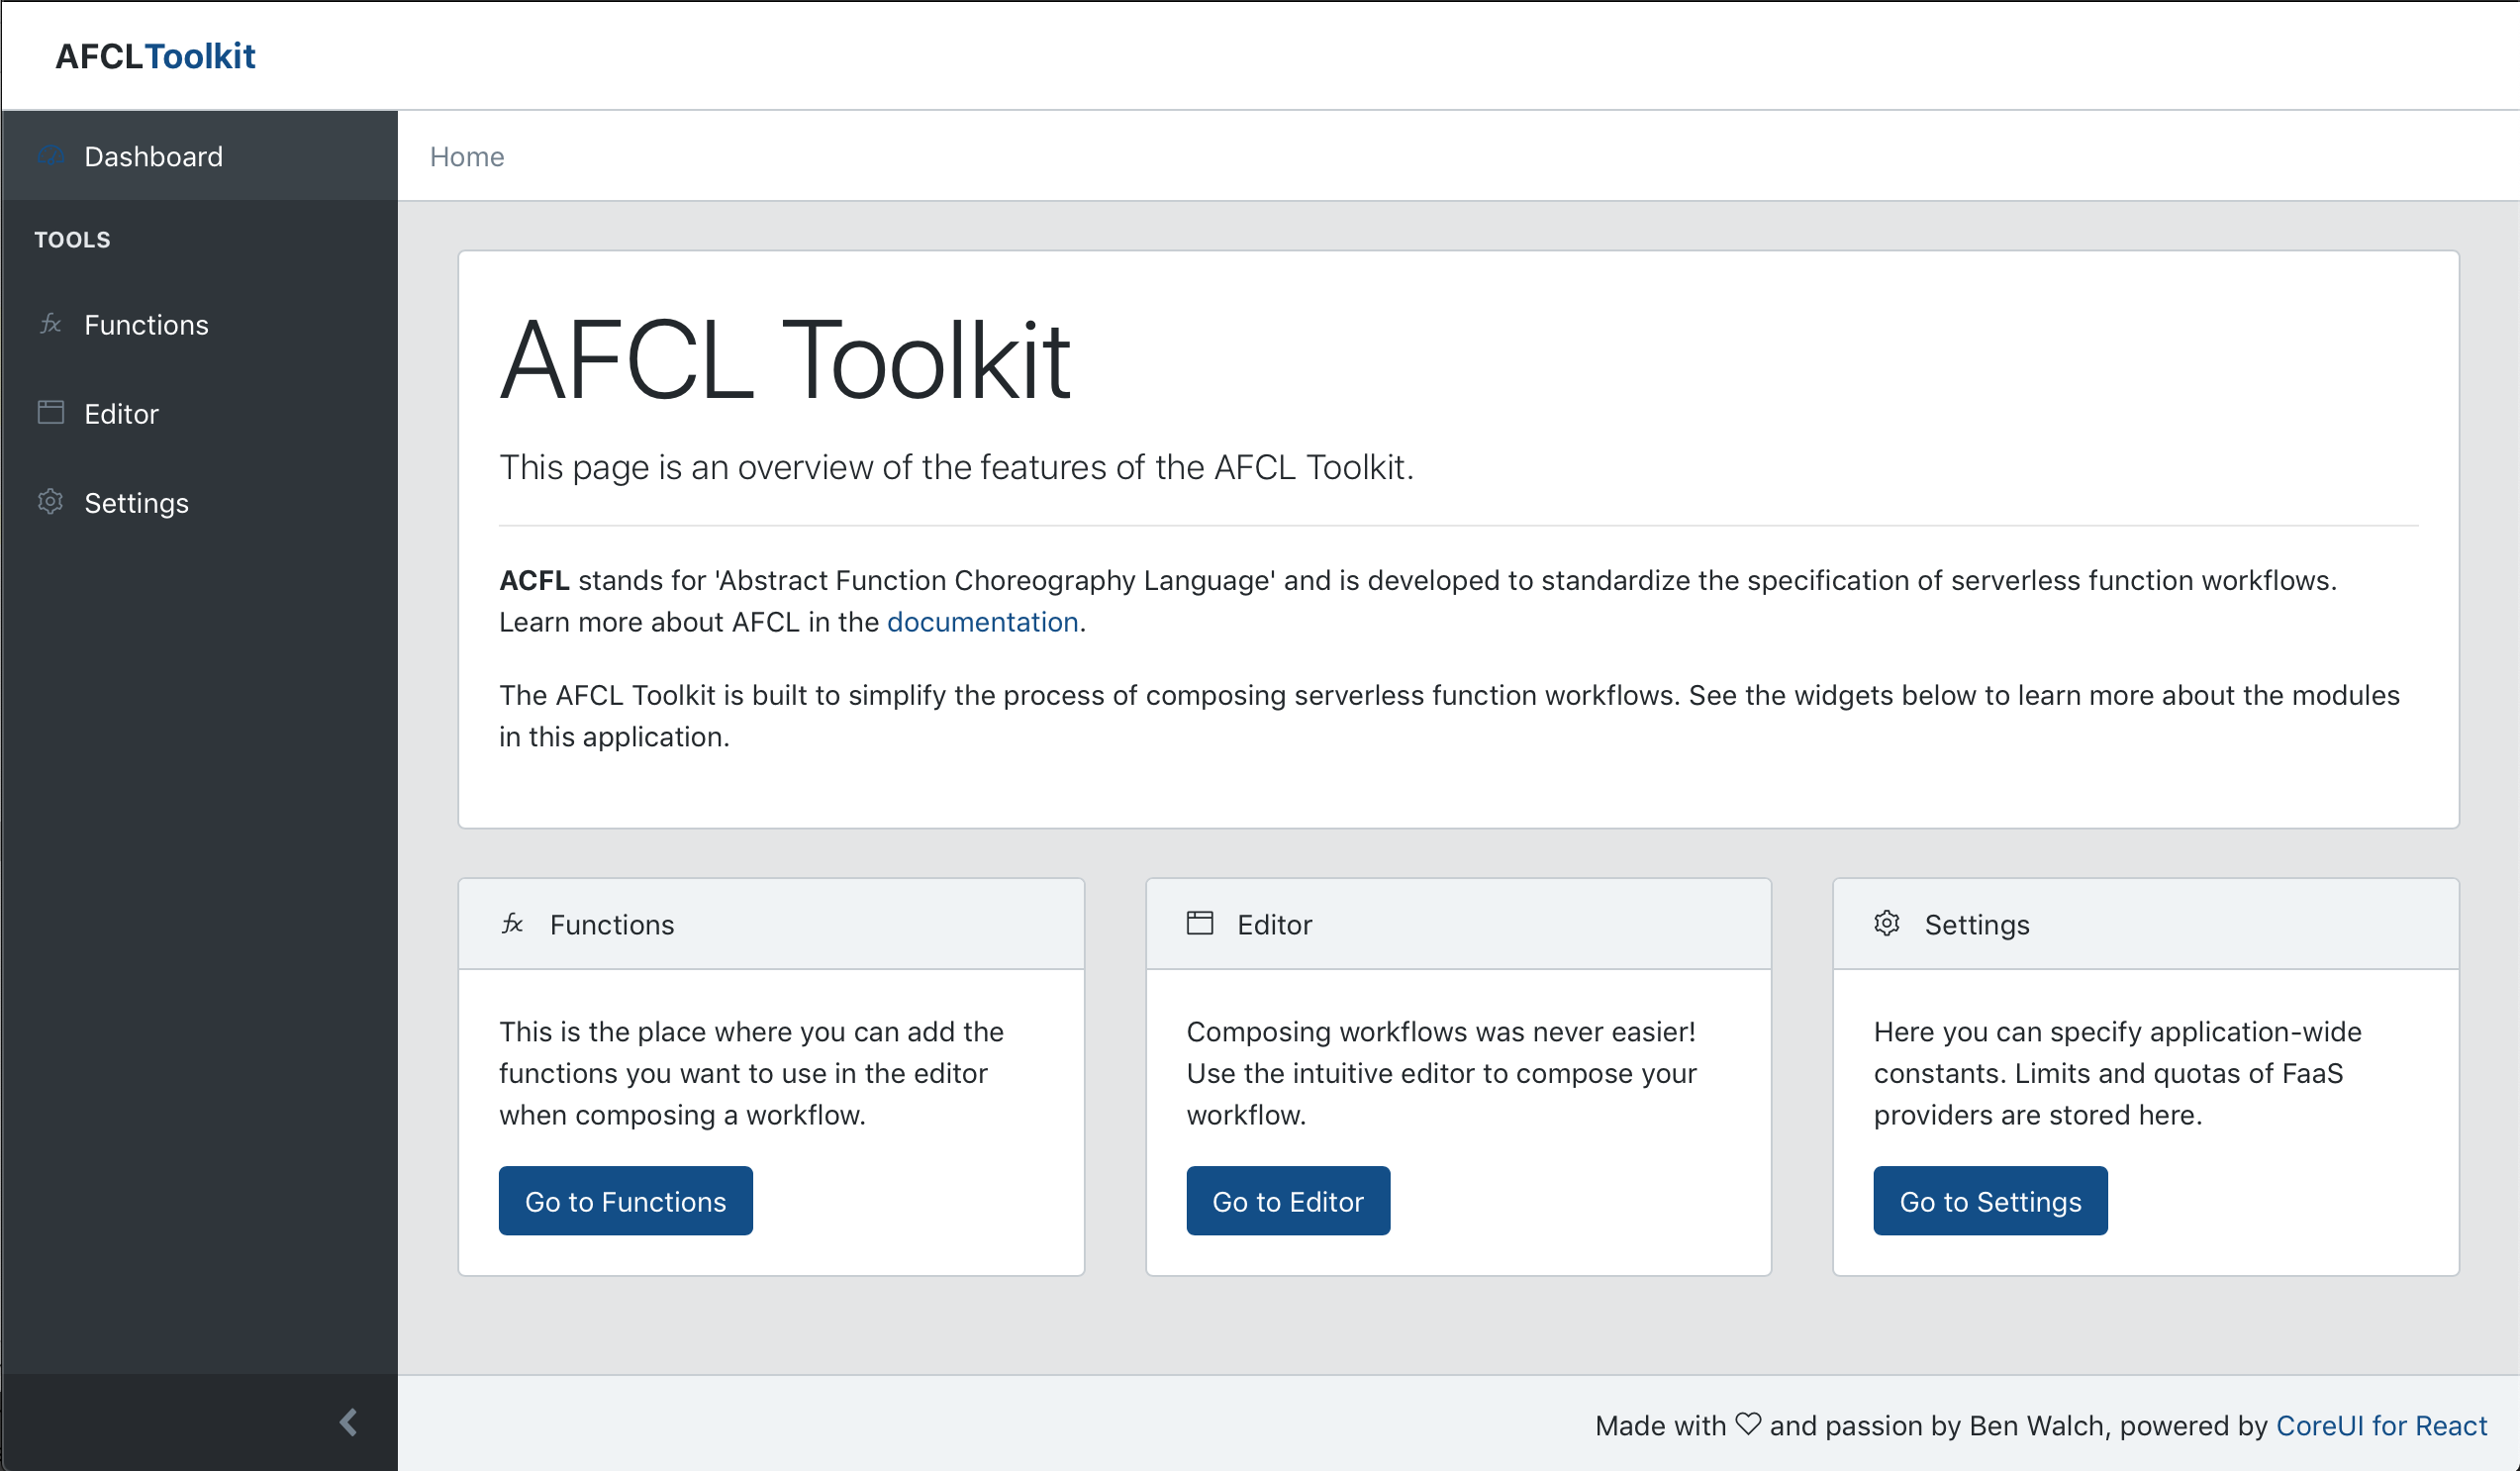
\includegraphics[width=\textwidth]{dashboard}
  \caption{the dashboard}
\end{figure}

\subsubsection{Functions}

A function repository is needed to know about available functions when composing a workflow. An item in the function repository holds the following data: name, type and provider. For In the implementation of this thesis, this data is persisted to an internal file.\footnote{see \ref{Backend-Persistence} for detailed information on how data is persisted}

\begin{figure}[ht]
  \centering
  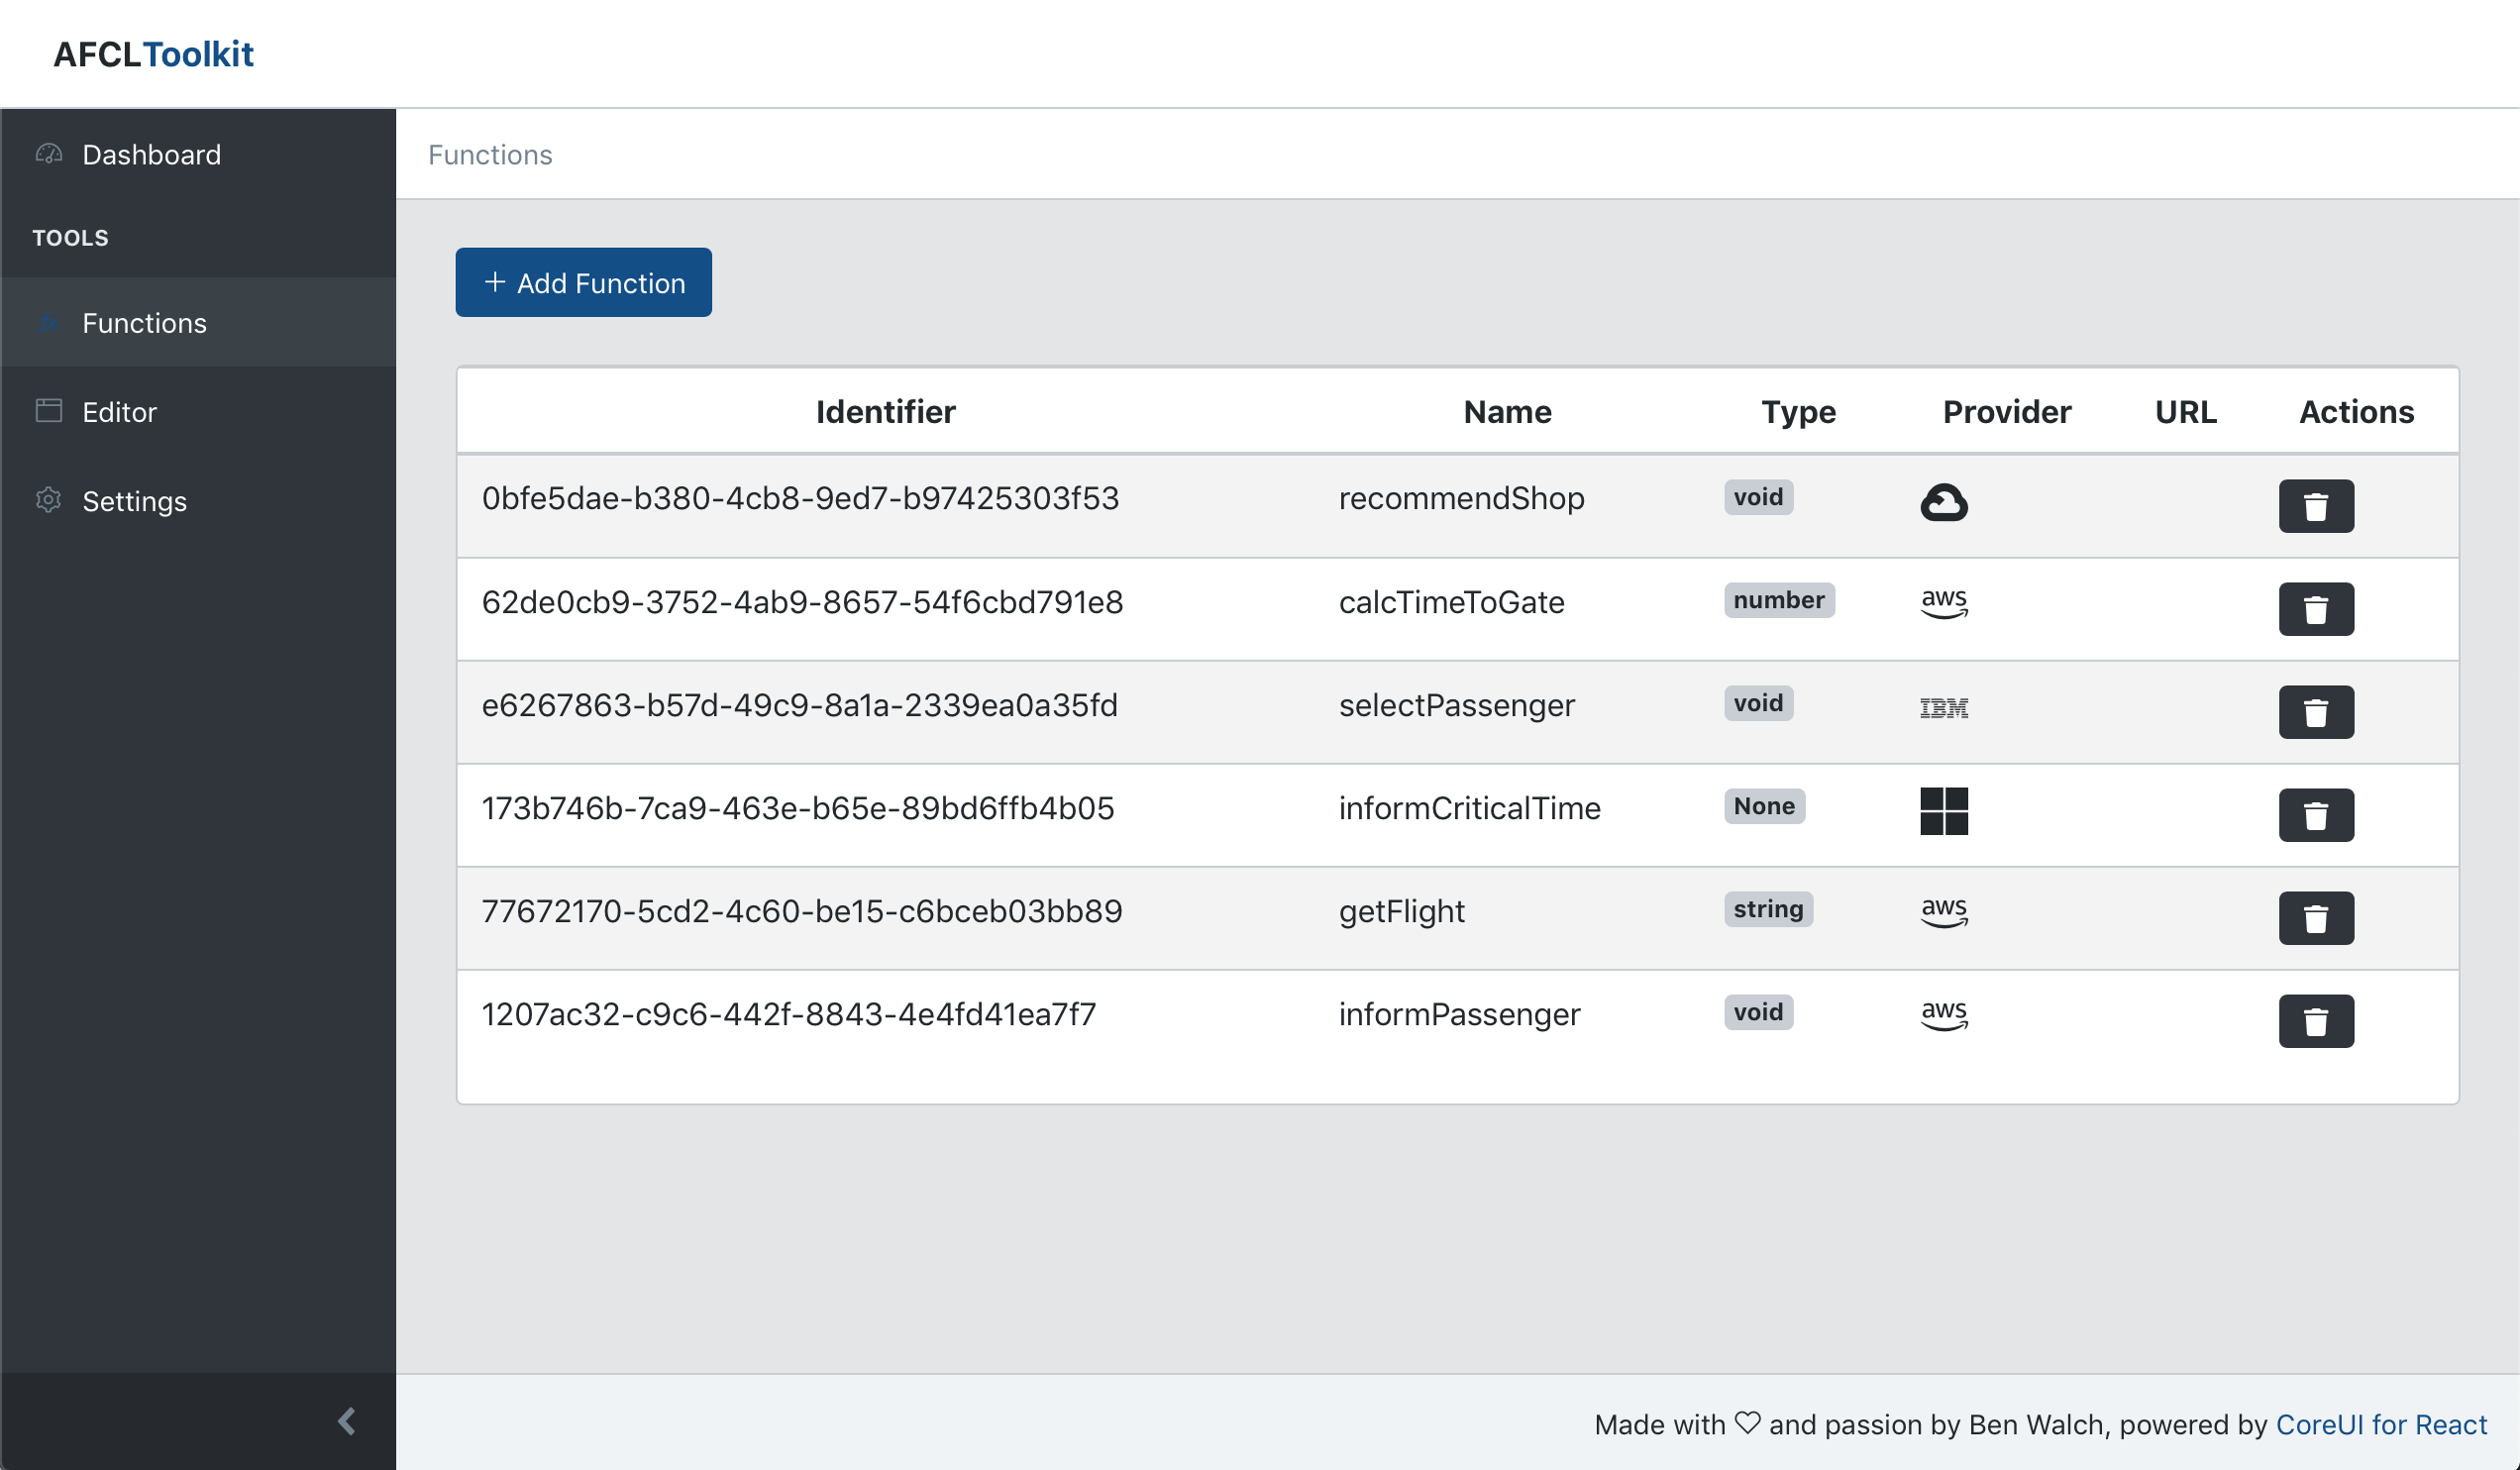
\includegraphics[width=\textwidth]{functions}
  \caption{the function repository}
\end{figure}

\subsubsection{Editor}
\par
The interface of the component for composing workflows is divided into two parts, on the left side is the editor, consisting of a toolbar and a drawing area. On the right side is the property view. In the editor, the user can choose a function from the toolbar to place it in the drawing area below.  For the sake of clarity, each function has a defined shape and style. In the drawing area, these shapes (functions) can then be connected to each other by drag and drop. This leads to a directed graph, which represent the execution flow. The possible connection points (ports) of a shape will be displayed when hovering over it. These ports are input and output for most of the functions. When hovering a port, the port name appears in the tooltip.
\par
When selecting a shape in the canvas, the property view changes. It displays each specific property of the selected function, with the ability to change, add or remove properties.

\begin{figure}[ht]
  \centering
  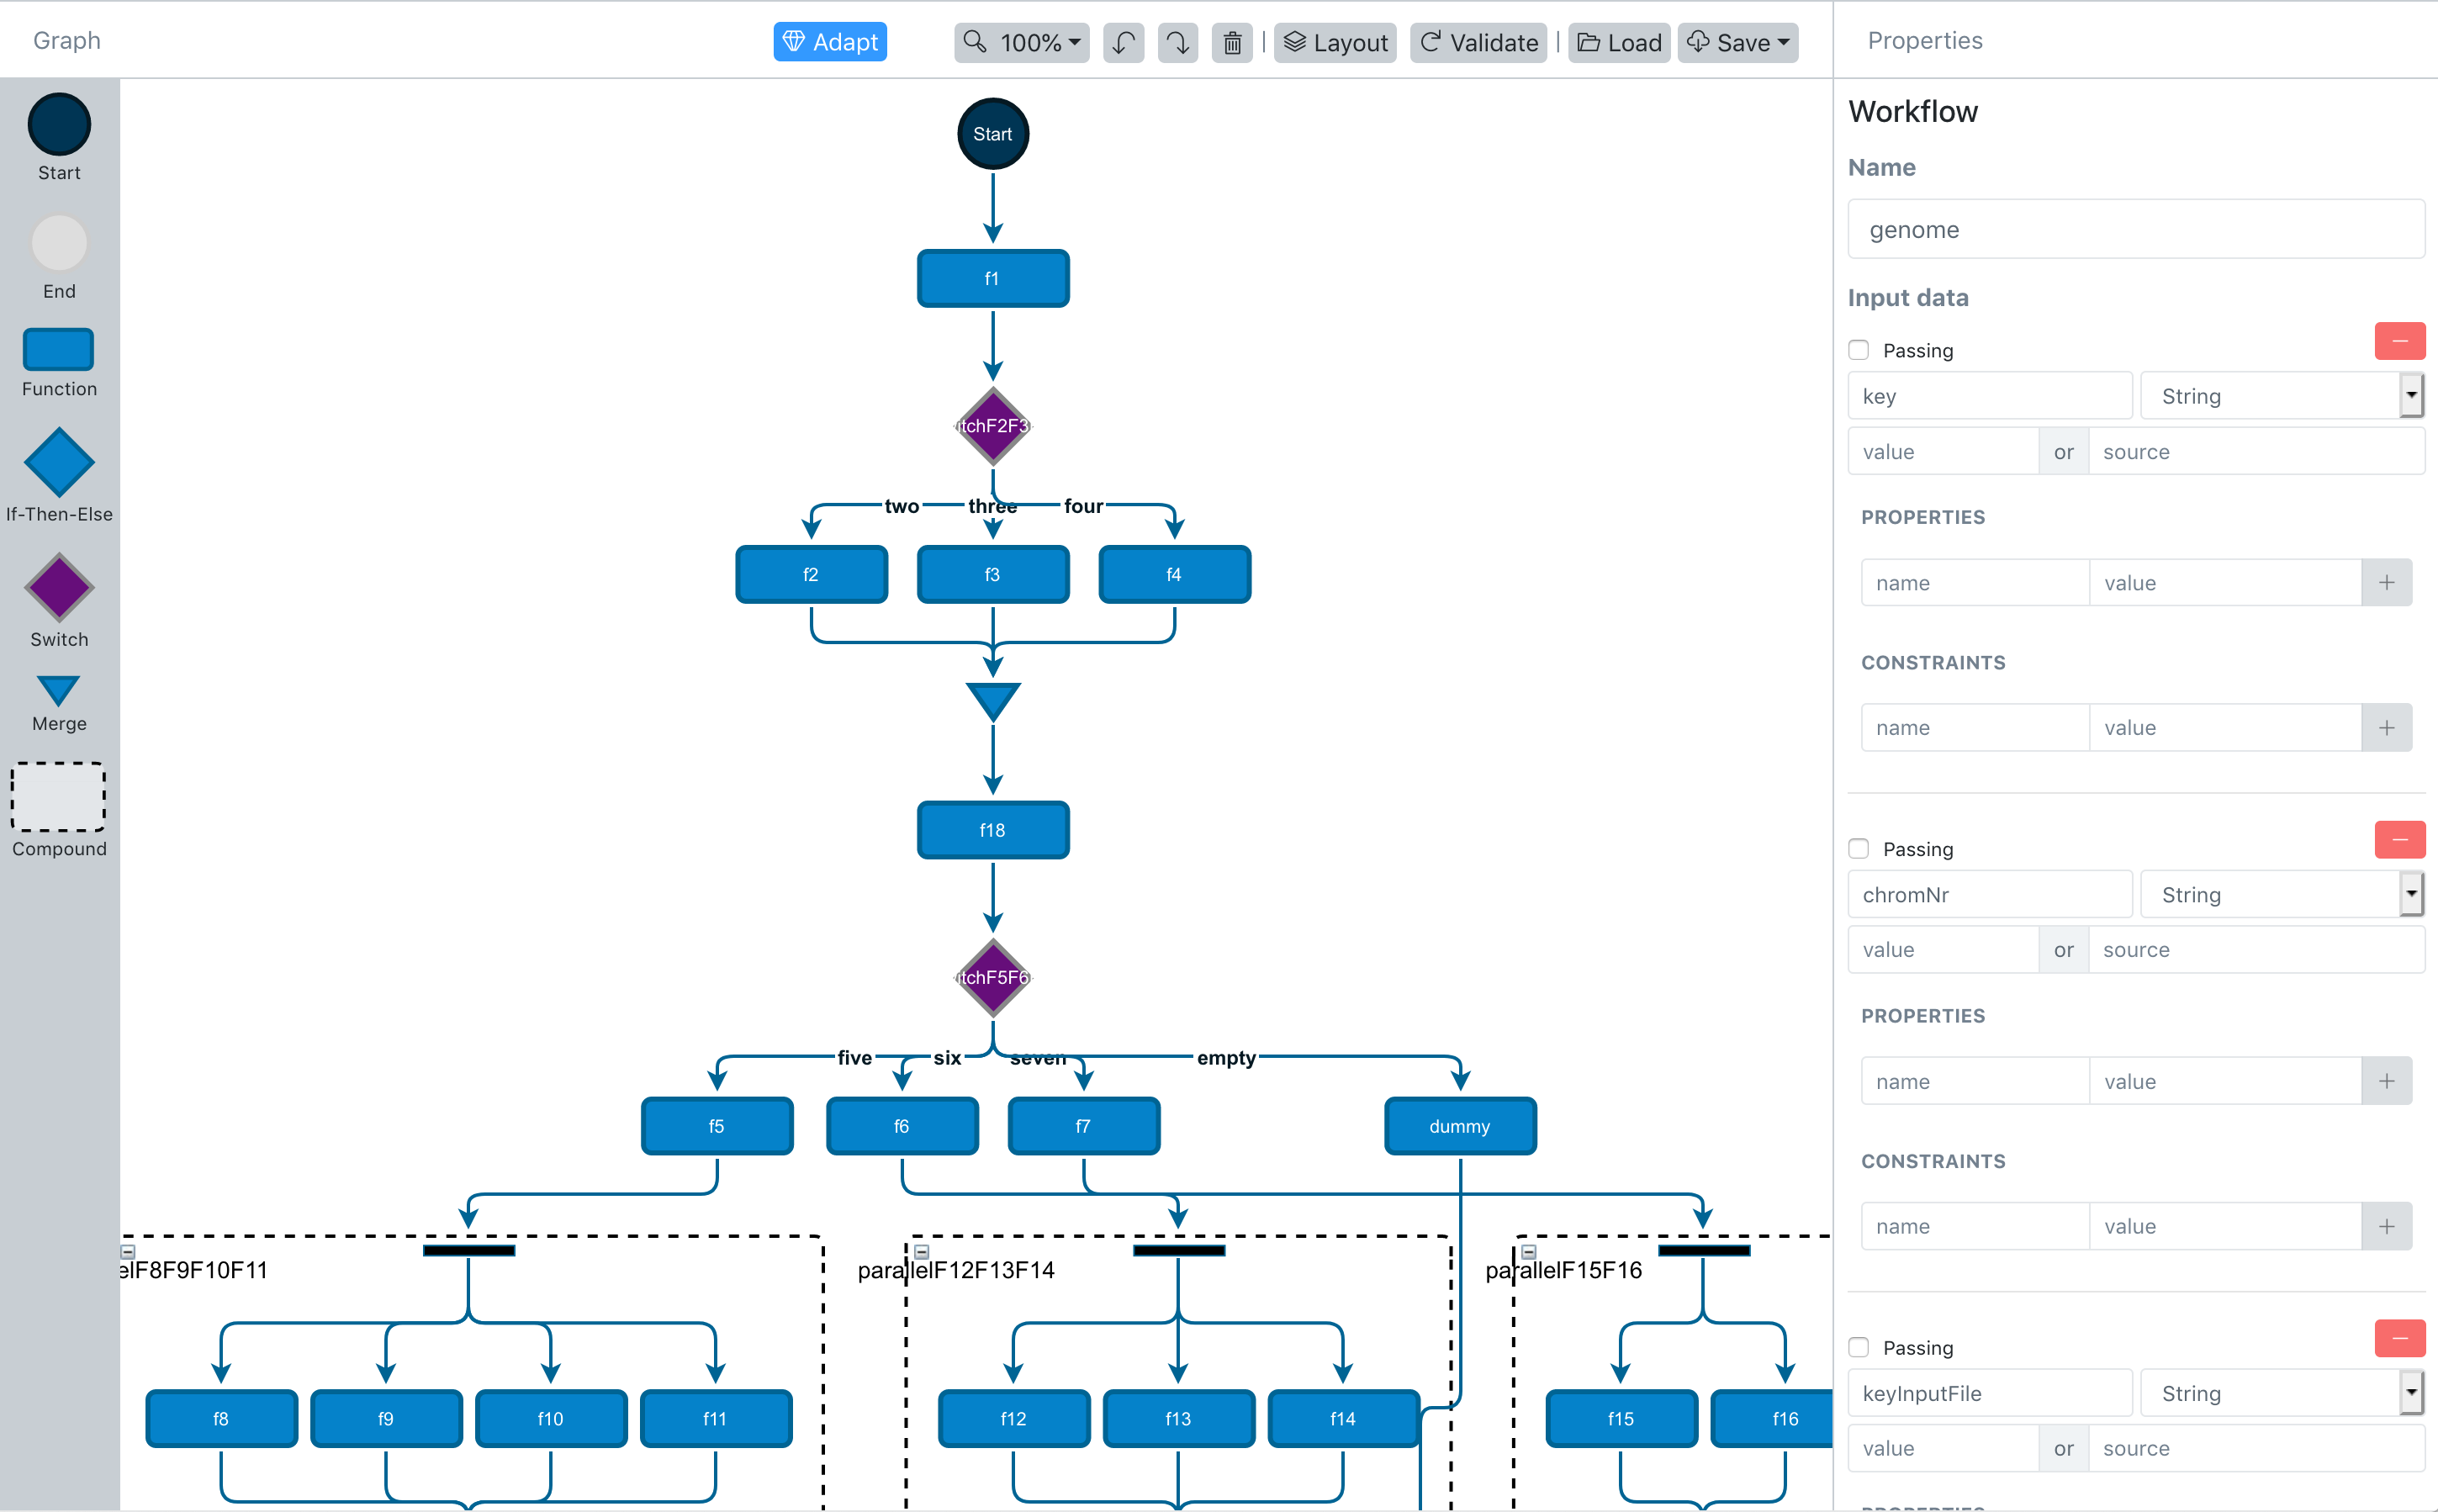
\includegraphics[width=\textwidth]{editor}
  \caption{the editor}
\end{figure}

\subsubsection{Graph}

% User Objects in Graph
% Validation
% Encoding

\subsubsection{Settings}

%% UI
%% Routing
%% React and Components
%% mxGraph and User Objects

\subsection{Backend}
\subsubsection{General}
\subsubsection{Maven}
\subsubsection{Servlets}
\subsubsection{Persistence}
\label{Backend-Persistence}

Composed workflows are be saved to the user's file system by offering a download. The user can then choose the target location.
The storing of function data, on the other hand, is abstracted from the user and persisting of the data is handled internally.
An interface\footnote{https://docs.oracle.com/javase/specs/jls/se7/html/jls-9.html} for the repository implementation was created on the backend side to be capable of supporting any data source. The repository which implements the interface in this thesis, stores the serialized data into a file. This could be easily replaced with any other implementation, for example an implementation which stores the data in a DBMS.

\subsubsection{Api}


\subsection{Continuous Delivery}

\section{Improvements}

\section{Conclusion}


% causes to print all bibliography
\nocite{*}

\bibliographystyle{IEEEtran}
\bibliography{thesis.bib}

\end{document} 
